\documentclass[12pt]{niuthesis}
% \documentclass[12pt,singlespacing]{niuthesis}

% some packages are loaded here
\usepackage{latexsym}		% to get LASY symbols
\usepackage{graphicx}		% to insert PostScript figures
\usepackage{rotating}           % defines sidways table and figure env.
\usepackage{hyperref}		% to insert hyperrefs
\hypersetup{
  bookmarksnumbered,
  bookmarksopen,
  bookmarksopenlevel=1,
  colorlinks=false,
  pdfborder={0 0 0},
  plainpages=true
}

%%%%%%%%%%%%%%%%%%%%%%%%%%%%%%%%%%%%%%%%%%%%%%%%%%%%%%%%%%%%%%%%
% Some LaTeX macros

\newcommand{\twochoices}[2]{\left\{ \begin{array}{lcc}
        \displaystyle #1 \\ \vspace{-10pt} \\
        \displaystyle #2 \end{array} \right. } %}

\newcommand{\twovec}[2]{\left(\begin{array}{c} #1 \\ #2 \end{array}\right)}

\newcommand{\twomatrix}[4]{\left(\begin{array}{cc} #1 & #2 \\ 
     #3 & #4 \end{array}\right)}

% Uncomment the following line for a List of Symbols
% \newcommand{\listofXXX}{\chapter*{List of Symbols}
\addcontentsline{toc}{chapter}{List of Symbols}

\begin{tabular}{cp{0.6\textwidth}}
  $x$ & position \\
  $v$ & velocity \\
  $a$ & acceleration \\
  $t$ & time \\
  $F$ & force
\end{tabular}\\
and many more!

\chapter*{List of Rockets}
\addcontentsline{toc}{chapter}{List of Rockets}

\begin{tabular}{cp{0.6\textwidth}}
  1232 & some old chinese rocekts \\
  1792 & rocket build by Hyder Ali \\
  1957 & R-7 (launched sputnik) \\
  1967 & Saturn V
\end{tabular}\\
and many more!

%%%%%%%%%%%%%%%%%%%%%%%%%%%%%%%%%%%%%%%%%%%%%%%%%%%%%%%%%%%%%%%%%%

%%% Local Variables: 
%%% TeX-master: "mythesis"
%%% End: 
}

%%%%%%%%%%%%%%%%%%%%%%%%%%%%%%%%%%%%%%%%%%%%%%%%%%%%%%%%%%%%%%%%%%
% Choose the chapter(s) / files you want to work with

%%% use this to compile all chapters
\def\files{ch1,ch2,refs,app1,app2}

%%% use this to work with only one chapter
% \def\files{ch2}

\includeonly{\files}

%%%%%%%%%%%%%%%%%%%%%%%%%%%%%%%%%%%%%%%%%%%%%%%%%%%%%%%%%%%%%%%%%
\begin{document}

\title{Five-Dimensional Flow in Solid\\ Fuel Rocket Engines\\
       -- Fun with \LaTeX}

\author{I.~B. Scriptor}

\major{Rocket Science}
\degree{Dissertation}{Ph.D.}{Doctor of Philosophy}
\degreedate{May}{2010}
\department{Department of Rocket Science}
\director{Wernher von Braun}

\begin{abstract}
  Solid fuel rocket engines are one of the most reliable and
  efficient propulsion systems used to lift payloads into orbit, in
  terms of $\lambda=(\Box+\Diamond)\psi$. Used throughout the
  astrodynamics community, the theory of the flow within the motor
  chamber is in fact a black art which defies all attempts at
  analysis.
	
  The present work (no exception to the statement above) contains a
  theoretical and numerical approach to the flow of the gases within
  the motor chamber. The shape of the chamber and original fuel
  configuration, and the patterns of combustion and flow/expulsion
  of gases, are modelled by a system of thirty fourth-degree
  differential equations.
  \begin{displaymath}
    f_i^{(34)}(x,y,z,t) = 
    \sum_{j=0}^{33} a_{ij} f_i^{(\mathrm{j})}(x,y,z,t)
  \end{displaymath}
  Acceptable numerical solutions would require one thousand pentium
  processors working day and night for $10^{11.2}$ years.
\end{abstract}

\begin{acknowledgments}
  Here's where you acknowledge folks who helped.
  Here's where you acknowledge folks who helped.
  Here's where you acknowledge folks who helped.
\end{acknowledgments}

\begin{dedication}
  To all of the fluffy kitties.
  To all of the fluffy kitties.
  To all of the fluffy kitties.
  To all of the fluffy kitties.
\end{dedication}

% comment this to suppress prologue
\MakeThesisPrologue % includes table of contents
% \tableofcontents

\chapter{Introduction}		% chapter 1
\label{introchap}		% for reference (\ref{introchap})

This sample document illustrates how to use the
{\tt niuthesis} class.
We always put a bit of text in between the heading commands to see how it goes.
\emph{We always put a bit of text in between the heading commands to see how it goes.}

\section{This Is a Section (Level 2)}

First we want to see how the sectioning commands work on different
levels of sectioning.
We always put a bit of text in between the heading commands to see how it goes.
\textbf{We always put a bit of text in between the heading commands to see how it goes.}

\subsection{So Here We Have a Subsection (Level 3)}

We always put a bit of text in between the heading commands to see how it goes.
We always put a bit of text in between the heading commands to see how it goes.
We always put a bit of text in between the heading commands to see how it goes.

\subsubsection{And Here a \LaTeX\ Subsubsection  (Level 4)}

We always put a bit of text in between the heading commands to see how it goes.
We always put a bit of text in between the heading commands to see how it goes.
We always put a bit of text in between the heading commands to see how it goes.

\paragraph{And Here Yet Lower Sectioning, a Paragraph (Level 5)}

We always put a bit of text in between the heading commands to see how it goes.
We always put a bit of text in between the heading commands to see how it goes.
We always put a bit of text in between the heading commands to see how it goes.

%% subparagraphs work fine. But they should not appear in an
%% official NIU thesis.
%% \subparagraph{Does anyone ever need subparagraphs?  (Level 6)} 

%% Well we provide subparagraphs anyway because they are part of \LaTeX.
%% We always put a bit of text in between the heading commands to see how it goes.
%% We always put a bit of text in between the heading commands to see how it goes.

\section{This Is a Section (Level 2)}

First we want to see how the sectioning commands work on different
levels of sectioning.
We always put a bit of text in between the heading commands to see how it goes.
We always put a bit of text in between the heading commands to see how it goes.

\section{This Is a Section (Level 2)}

First we want to see how the sectioning commands work on different
levels of sectioning.
We always put a bit of text in between the heading commands to see how it goes.
We always put a bit of text in between the heading commands to see how it goes.

\section{This Is a Long Section Title That Needs to Be Broken Over
 Two Lines -- or May Be Three? We Will See $\ldots$}

Some requirements of the Graduate School are written
into that file; page size, line spacing, appropriate
placement of captions for tables and figures, etc.
Other tasks of conforming to the requirements are
left to other existing \LaTeX{} packages.

\subsection{Question:  What Are the Issues in Studying This Subject?}

A major goal in studying solid fuel rocket motors is to create a model
of the dynamics of a motor chamber.  This involves two major goals:
the combustion zone and the acoustic zone.

The combustion zone consists of the thin layer above the solid fuel
where the gasification of the fuel takes places. The zone is very
reactive and highly turbulent. The acoustic-vortical zone is the
volume of gas above the combustion zone. Within this zone, the gas
is non-reactive and contains acoustic waves and vorticity. The work
presented here\footnote{Footnotes are handled neatly by \LaTeX.} is
an extension of Lao \cite{lao:thesis} and Lao et~al.\
\cite{lao:paper}. The driving frequency is on the order of the
inverse of the axial acoustic time scale, $t_A'= L'/C_0'$, where
$L'$ is the length of the cylinder and $C_0'$ is the reference speed
of sound.\footnote{Remember the traditional method of calculating
 the distance of lightning? See the flash, count seconds until you
 hear the thunder, divide by five, that's the number of miles. That
 assumes $C_0=\frac{1 mi.}{5 s}$.} Radial and azimuthal velocities
are found to vanish exponentially fast in the downstream direction,
as suggested by Table \ref{powertable}.

\begin{table}[htb]
\caption[Example of a table with its own footnotes]{\label{powertable}
	Here is an example of a table with its own footnotes.
	Don't use the $\backslash${\tt footnote} macro if you
	don't want the footnotes at the bottom of the page.
	Also, note that in a thesis the caption goes
	\emph{above} a table, unlike figures.
	}
\begin{center}
\begin{tabular}{||l|c|c|c|c||} \hline
	& $S$ & $P$ &   $Q^{\ast}$  & $D^{\dagger}$ \\	% footnote symbols!
	wave form & (kVA) & (kW) & (kVAr) & (kVAd) \\  \hline \hline
	& 25.87 & 25.83 & 1.3 & $\approx 0$ \\ \hline
	& 25.48 & 25.00 & -2.82 & 4.03 \\ \hline
	& 25.11 & 18.02 & -9.75 & 14.52 \\ \hline
	Table \ref{tbl:sample2}  & 24.98 & 22.26 & 9.19 & 6.64 \\ \hline
	Fig.  \ref{tbl:sidewaysT}  & 23.48 & 15.00 & 6.59 & 16.82 \\ \hline
	Fig.  \ref{fig:pyramid}  & 24.64 & 22.81 & -0.44 & 9.3 \\ \hline
	Fig.  \ref{fig:sidewaysF}  & 23.03 & 18.01 & 3.36 & 13.95 \\ \hline
	\end{tabular}
   \\ \rule{0mm}{5mm}
   ${}^\ast$kVAr means reactive power.		% footnote symbol
\\ ${}^\dagger$kVAd means distortion power.	% footnote symbol
\end{center}
\end{table}

These results provide an analytical explanation of those
found from computational analysis by Fabnis
et~al.\ \cite{fabnis}.  The non-axisymmetric flow near the
endwall contains cross-sectional velocity patterns that
include flow across the cylinder axis.  A viscous boundary
layer adjacent to the sidewall and near the endwall is
studied to find the transition between the transient core
flow and the no-slip condition on the sidewall.
It is found, as in Lao et~al.\ \cite{lao:paper}, that the
azimuthal component of the vorticity is proportional to
the inverse of the Mach number.  In addition, the axial
component of the vorticity driven by the non-axisymmetric
boundary condition at the endwall is also found to be
proportional to the the inverse of the Mach number.

%%%%%%%%%%%%%%%%%%%%%%%%%%%%%%%%%%%%%%%%%%%%%%%%%%%%%%%%%%%%%%%%%%

%%% Local Variables: 
%%% TeX-master: "mythesis"
%%% End: 
		% file with Chapter 1 contents
\chapter{Mathematical Formulation}
\label{mathchapter}

The objective of this fake thesis document is to demonstrate some
\LaTeX{} features as well as features specific to the thesis class.
We start by giving one short formula, 
\begin{equation}
	A = \pi r^2,
\end{equation}
and one big hairy multi-line
formula (one of the non-dimensional Navier-Stokes equations):
\begin{eqnarray}
  \rho \left[ \frac{DV_r}{Dt} - M \epsilon^2
    \frac{V_\theta^2}{r} \right]
  & = & -\frac{\delta^2}{\gamma~ M} \frac{\partial P}{\partial r}
	+ \frac{M ~\delta^2}{Re} \left\{ 2 \frac{\partial }{\partial r}
	\left[ \mu \left( \frac{\partial V_r}{\partial r}
        - \frac{1}{3} {\bf \nabla \cdot \overline{V}}
      \right) \right] \right. \nonumber \\
  & & + \frac{1}{r} \frac{\partial }{\partial \theta} \left[ \mu \left(
      \frac{1}{r} \frac{\partial V_r}{\partial \theta} + \epsilon \frac{\partial V_{\theta}}{\partial r}
      - \epsilon \frac{V_{\theta}}{r} \right) \right] \nonumber \\
  & & + \frac{\partial }{\partial z} \left[ \mu \left( \frac{1}{\delta^2}
        \frac{\partial V_r}{\partial z} + \frac{\partial V_z}{\partial r} \right) \right] \nonumber \\
  & & + 2 \left. \frac{\mu}{r}\left[ \frac{\partial V_r}{\partial r} -\frac{\epsilon}{r}
      \frac{\partial V_{\theta}}{\partial \theta} - \frac{V_r}r\right] \right\}, \label{eq:rmom}
\end{eqnarray}
The latter equation is non-dimensionalized using the following definitions:
\begin{displaymath}
	r = \frac{r'}{R'}, \quad
	z = \frac{z'}{L'}, \quad
	t = \frac{t'}{t_a'}, \quad
	\kappa = \frac{\kappa'}{\kappa_0'}, \quad
	\mu = \frac{\mu'}{\mu_0'} , \quad
	C_V = \frac{C_V'}{C_{V0}'},
      \end{displaymath}
where $P_0'$ is the initial static pressure in the cylinder,
and $\rho_0'$ and $T_0'$ are the density and temperature
of the fluid being injected from the sidewall.
The aspect ratio is given by $\delta = \frac{L'}{R'}$,
where $\delta \gg 1$.
The induced characteristic axial velocity and the characteristic
endwall velocity disturbance $V_{z0}'$ is defined with respect
to the injection reference sidewall velocity,
$V_{r0}'$ by overall mass conservation,
$\frac{V_{z0}'}{V_{r0}'} = \delta$.
The size of the initially unknown reference
azimuthal velocity $V_{\theta 0}'$ is related to
$V_{r0}'$ by $\frac{V_{\theta 0}'}{V_{r0}'}=\epsilon$.
Later, it is shown that $\epsilon=1$.

\begin{figure}
\centerline{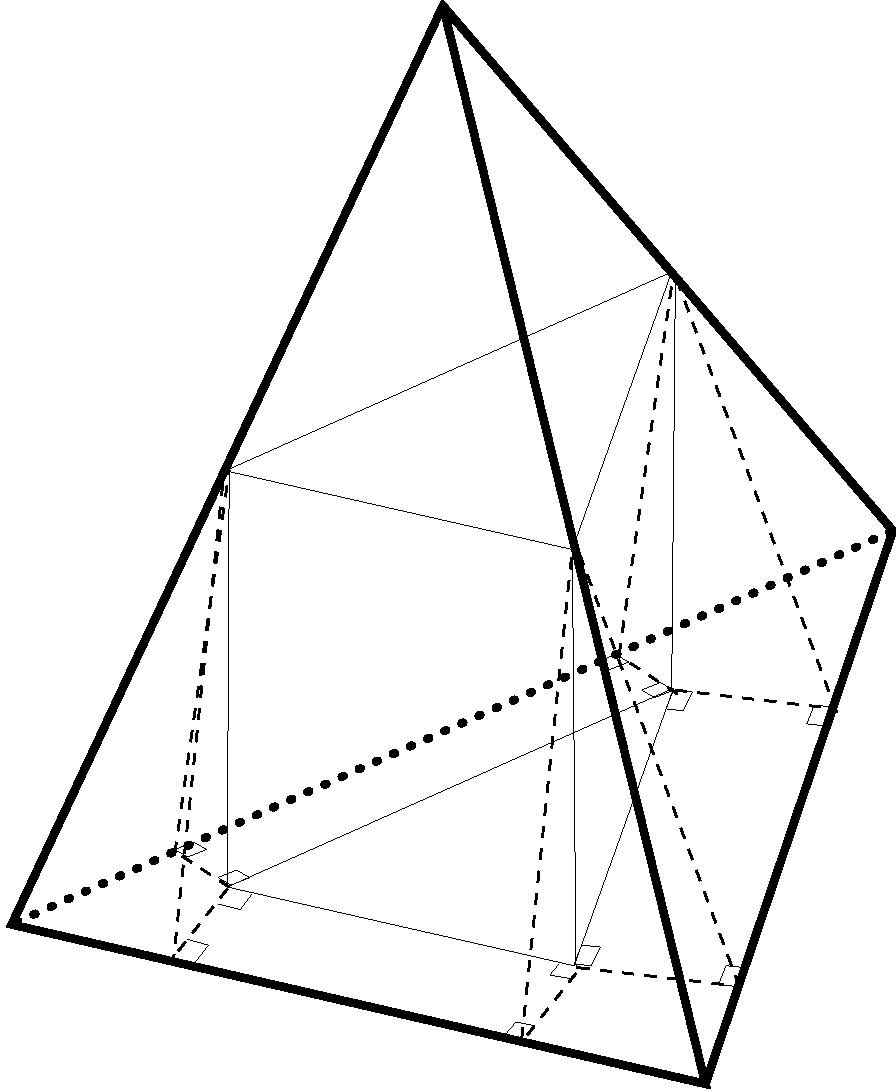
\includegraphics[height=95mm]{pyr}}
\caption[Cutting up a triangular pyramid]{
	A triangular pyramid may be cut up as shown, to
	yield one top pyramid (with one-eighth the volume
	of the full pyramid), three bottom corner pyramids
	(which, when joined, are congruent to the top pyramid),
	three prisms along the bottom edges (the area of whose
	bottom faces total $B/2$) and the large central prism
	(volume = $(B/4)(h/2) = Bh/8$).
	The image, from PostScript file ``pyr.eps'',
	was read in using the {\tt $\backslash$includegraphics}
	command, from the {\tt graphicx} package.
	}
\label{fig:pyramid}
\end{figure}

The time is non-dimensionalized using the
axial acoustic time scale,
$t_a'=\frac{L'}{C_0'}$, where
$C_0'=(\gamma {\cal R} ' T_0')^{\frac12}$
is the speed of
sound,\footnote{In air at 1 atm., $\frac{1 mi.}{5 s}$.}
$\cal{R}'$ is the gas constant,
and $\gamma$ is the ratio of specific heats.
Also the Reynolds number, Wrenchl number,
and Mock number are defined as
\begin{displaymath}
	Re = \frac{\rho' V_{z_0}' L'}{ \mu_0'}, \quad
	Wr = \frac{\mu_0' C_{p_0}'}{\kappa_0'}, \quad
	M = \twovec{V_{z_0}'}{C_0'} \cdot
		\twomatrix{8a}{z_0-\rho}2{z_0-\mu} \twovec{Wr}{p-7},
\end{displaymath}
where $Re\ll1$, $M\gg1$, and $Wr=O(1)$.

Here is an example of using the \texttt{singlespace} environment.

\begin{singlespace}
  This paragraph was surrounded by the \texttt{singlespace}
  environment. The Mock number is chosen as a small parameter to
  model the small magnitude found in a typical rocket motor chamber,
  as opposed to the rocket nozzle where larger values are
  possible.\footnote{Not just possible, desirable!} The aspect
  ratio, $\delta$, is taken to be a large parameter, because many
  chambers have aspect ratios between 15 and 50.
\end{singlespace}

The following table is created using the \LaTeX{}
\texttt{tabular} environment.

\begin{table}
\begin{center}
\label{tbl:sample2}
\caption[Yet another {\tt tabular} table]{
	This is a table constructed with \LaTeX{}
	commands in the {\tt tabular} environment.
	}
   \begin{tabular}{|c||c|c|c|c||c|} \hline
   n & $n^2$ & $n^3$ & $n^4$  & $n^7$ & $n^{13}$ \cr \hline \hline
   2 &  4  &  8  &   16    &    128  & 8192 \cr
   3 &  9  &  27  &   81    &   2187  & 1594323 \cr \hline
   4 &  16  &  64  &   256   &  16384  & 67108864 \cr
   5 &  25  &  125  &   625  &  78125  & 1220703125 \cr \hline
   6 &  36  &  216  &   1296 &  279936  & 13060694016 \cr
   7 &  49  &  343  &   2401 &  823543  & 96889010407 \cr \hline
   \end{tabular}
\end{center}
\end{table}

However, sometimes you want to use a table produced by some other
software, such as Excel.  If the table is saved to a PostScript file,
then it can be displayed using the $\backslash${\tt includegraphics}
macro inside a {\tt table} environment:

\begin{table}
  \caption[Table from a PostScript file]{\label{tbl:sample3}
   Table from a PostScript file. This table wasn't constructed with
   \LaTeX\ commands, but resides in a PostScript file
   ({\tt tableD.eps}) created by some other software.}
  \vspace{2ex}
  \centerline{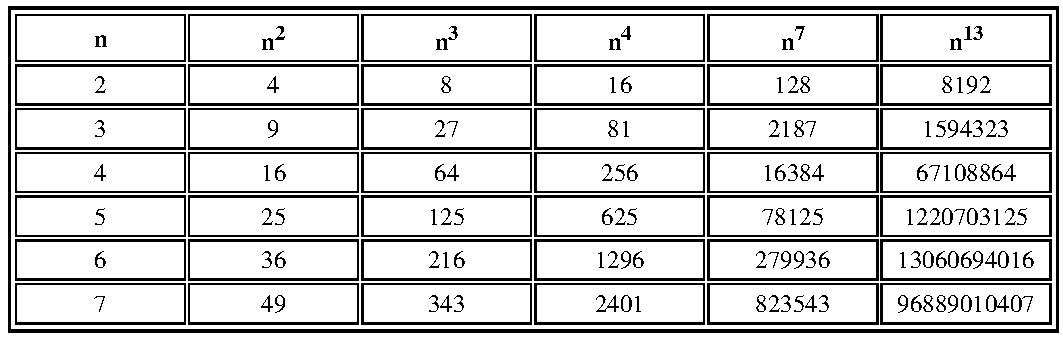
\includegraphics[width=\textwidth]{tableD}}
\end{table}

\section{Conditions for Catastrophic Combustion}
\label{sec:cata}

Initially, a steady flow is generated by the sidewall injection,
$V_r = -V_{rws}(z)$. The subscript $srw$ is used to mean that there
is a {\bf s}teady {\bf r}adial {\bf w}all velocity. The sign is
negative due to the injection toward centerline. At $t=0^+$, the
endwall begins oscillating with the non-dimensionalized sinusoidal
axial velocity, $V_z=\widetilde{F}_{rw}(r,\theta,t)$, for $\omega =
O(1)$.

Some of the boundary conditions are:
\begin{eqnarray}
  z=0; && V_z = \twochoices
	{0, && t\leq0}
	{\widetilde{F}_{zw}(r,\theta,t), && t>0}
						\label{eq:endwall} \\
  z=0; && V_{\theta}=V_r=0,			\label{eq:endnoslip} \\
  r=0; && P,\rho,T,V_r,V_{\theta},V_z~\mbox{finite},	\label{eq:centerline} \\
  r=1; && V_r= F_{rws}(z),			\label{eq:injection} \\
  r=1; && V_z=V_{\theta} =0,				\label{eq:sidenoslip}
\end{eqnarray}
and solutions must be periodic in $\theta$.


\section{More Boundary Conditions}
\label{sec:bcs}

Initially, a steady flow is generated by the
sidewall injection, $V_r = -V_{rws}(z)$.
The sign is negative due to the injection toward
centerline.\footnote{This convention was
suggested by Goddard and Smythe.}
At $t=0^+$, the endwall begins oscillating with the
non-dimensionalized sinusoidal axial velocity,
$V_z =\widetilde{F}_{rw}(r,\theta,t)$,
for $\omega = O(1)$.
The frequency condition chosen represents the
first few axial acoustic modes observed in high
aspect ratio chambers.\footnote{Toy rockets,
the kind you used to shoot off with your dad
in the park, typically have only two significant
modes.}

The full boundary conditions include:
\begin{eqnarray}
  z=0; && V_{\theta}=V_r = 0,            \label{eqB:endnoslip} \\
  r=1; && V_r= \left\{
    \begin{array}{ll}
      F_{rws}(z), & t<0, \\
      F_{rws}(z)+\widetilde{F}_{rw}(z,\theta,t), & t\geq 0
    \end{array}
  \right.                               \label{eqB:injection} \\
  r=1; && V_z=V_{\theta} =0,                  \label{eqB:sidenoslip}
\end{eqnarray}
and solutions must be periodic in $\theta$.

If you don't believe this stuff, check out
Mulick \cite{mulick} and Baylor \cite{baylor}.

\subsection{Just Meaningless Text to Test Lines per Page
	\label{ss}}

Just meaningless text to test lines per page.
Just meaningless text to test lines per page.
Just meaningless text to test lines per page.
Just meaningless text to test lines per page.
Just meaningless text to test lines per page.
Just meaningless text to test lines per page.
Just meaningless text to test lines per page.
Just meaningless text to test lines per page.
Just meaningless text to test lines per page.
Just meaningless text to test lines per page.
Just meaningless text to test lines per page.
Just meaningless text to test lines per page.
Just meaningless text to test lines per page.
Just meaningless text to test lines per page.
Just meaningless text to test lines per page.
Just meaningless text to test lines per page.
Just meaningless text to test lines per page.
Just meaningless text to test lines per page.
Just meaningless text to test lines per page.
Just meaningless text to test lines per page.
Just meaningless text to test lines per page.
Just meaningless text to test lines per page.
Just meaningless text to test lines per page.
Just meaningless text to test lines per page.
Just meaningless text to test lines per page.
Just meaningless text to test lines per page.
Just meaningless text to test lines per page.
Just meaningless text to test lines per page.
Just meaningless text to test lines per page.
Just meaningless text to test lines per page.
Just meaningless text to test lines per page.
Just meaningless text to test lines per page.
Just meaningless text to test lines per page.
Just meaningless text to test lines per page.
Just meaningless text to test lines per page.
Just meaningless text to test lines per page.
Just meaningless text to test lines per page.
Just meaningless text to test lines per page.
Just meaningless text to test lines per page.
Just meaningless text to test lines per page.
Just meaningless text to test lines per page.
Just meaningless text to test lines per page.
Just meaningless text to test lines per page.
Just meaningless text to test lines per page.
Just meaningless text to test lines per page.
Just meaningless text to test lines per page.
Just meaningless text to test lines per page.
Just meaningless text to test lines per page.
Just meaningless text to test lines per page.
Just meaningless text to test lines per page.
Just meaningless text to test lines per page.
Just meaningless text to test lines per page.
Just meaningless text to test lines per page.
Just meaningless text to test lines per page.
Just meaningless text to test lines per page.
Just meaningless text to test lines per page.
Just meaningless text to test lines per page.
Just meaningless text to test lines per page.
Just meaningless text to test lines per page.
Just meaningless text to test lines per page.
Just meaningless text to test lines per page.
Just meaningless text to test lines per page.
Just meaningless text to test lines per page.
Just meaningless text to test lines per page.
Just meaningless text to test lines per page.
Just meaningless text to test lines per page.
Just meaningless text to test lines per page.
Just meaningless text to test lines per page.
Just meaningless text to test lines per page.
Just meaningless text to test lines per page.
Just meaningless text to test lines per page.
Just meaningless text to test lines per page.
Just meaningless text to test lines per page.
Just meaningless text to test lines per page.
Just meaningless text to test lines per page.
Just meaningless text to test lines per page.
Just meaningless text to test lines per page.
Just meaningless text to test lines per page.
Just meaningless text to test lines per page.
Just meaningless text to test lines per page.
Just meaningless text to test lines per page.
Just meaningless text to test lines per page.
Just meaningless text to test lines per page.
Just meaningless text to test lines per page.

\subsection{This Is a Subsection}

This is a subsection.
Filler filler filler filler filler filler filler filler.
Filler filler filler filler filler filler filler filler.

\subsection{This Is Another Subsection}

This is another subsection.
Filler filler filler filler filler filler filler filler.
Filler filler filler filler filler filler filler filler.

\paragraph{This Is a Paragraph}
It used a \verb2\paragraph{}2 header, which
are always inlined (with extra space)
and  boldfaced.

Filler filler filler filler filler filler filler filler.
Filler filler filler filler filler filler filler filler.

\paragraph{What Is It?}
This is a paragraph.
The heading of the paragraph is emphasized.
This is a paragraph.
The heading of the paragraph is emphasized.

\section{Sideways Tables}

In Table~\ref{tbl:sidewaysT} on page~\pageref{tbl:sidewaysT} we show
on a separate page how \LaTeX\ can handle big tables that need to be
put sideways. All we need to do is to put the table into a
\texttt{sidewaystable} environment. The rest is handled by \LaTeX.
In particular, we can easily make sure that the table will take just
the available space. That's neat, isn't it? Just make sure you load
the \texttt{rotating} package that defines the
\texttt{sidewaystable} environment.

\begin{sidewaystable}[ht]
  \caption{\label{tbl:sidewaysT}A big table that needs to go
   sideways -- easy with \LaTeX.}

  \vspace{2ex}
  \renewcommand{\arraystretch}{1.2}
  \begin{tabular*}{\textwidth}{@{\extracolsep{\fill}}*{26}{r}}
    \hline\hline
    a & b & c & d & e & f & g & h & i & j & k & l & m & n & o &
     p & q & r & s & t & u & v & w & x & y & z
    \\ \hline
    1 & 2 & 3 & 4 & 5 & 6 & 7 & 8 & 9 &
    10 & 11 & 12 & 13 & 14 & 15 & 16 & 17 & 18 & 19 &
    20 & 21 & 22 & 23 & 24 & 25 & 26 \\
    26 & 25 & 24 & 23 & 22 & 21 & 20 &
    19 & 18 & 17 & 16 & 15 & 14 & 13 & 12 & 11 & 10 &
    9 & 8 & 7 & 6 & 5 & 4 & 3 & 2 & 1 \\
    1 & 2 & 3 & 4 & 5 & 6 & 7 & 8 & 9 &
    10 & 11 & 12 & 13 & 14 & 15 & 16 & 17 & 18 & 19 &
    20 & 21 & 22 & 23 & 24 & 25 & 26 \\
    26 & 25 & 24 & 23 & 22 & 21 & 20 &
    19 & 18 & 17 & 16 & 15 & 14 & 13 & 12 & 11 & 10 &
    9 & 8 & 7 & 6 & 5 & 4 & 3 & 2 & 1 \\
    1 & 2 & 3 & 4 & 5 & 6 & 7 & 8 & 9 &
    10 & 11 & 12 & 13 & 14 & 15 & 16 & 17 & 18 & 19 &
    20 & 21 & 22 & 23 & 24 & 25 & 26 \\
    26 & 25 & 24 & 23 & 22 & 21 & 20 &
    19 & 18 & 17 & 16 & 15 & 14 & 13 & 12 & 11 & 10 &
    9 & 8 & 7 & 6 & 5 & 4 & 3 & 2 & 1 \\
    1 & 2 & 3 & 4 & 5 & 6 & 7 & 8 & 9 &
    10 & 11 & 12 & 13 & 14 & 15 & 16 & 17 & 18 & 19 &
    20 & 21 & 22 & 23 & 24 & 25 & 26 \\
    26 & 25 & 24 & 23 & 22 & 21 & 20 &
    19 & 18 & 17 & 16 & 15 & 14 & 13 & 12 & 11 & 10 &
    9 & 8 & 7 & 6 & 5 & 4 & 3 & 2 & 1 \\
    1 & 2 & 3 & 4 & 5 & 6 & 7 & 8 & 9 &
    10 & 11 & 12 & 13 & 14 & 15 & 16 & 17 & 18 & 19 &
    20 & 21 & 22 & 23 & 24 & 25 & 26 \\
    26 & 25 & 24 & 23 & 22 & 21 & 20 &
    19 & 18 & 17 & 16 & 15 & 14 & 13 & 12 & 11 & 10 &
    9 & 8 & 7 & 6 & 5 & 4 & 3 & 2 & 1 \\
    \hline \hline
   \end{tabular*}
\end{sidewaystable}

\section{Sideways Figures}

The \texttt{rotating} package also defines a \texttt{sidewaysfigure}
environment. This works well with big figures -- convince yourself
by looking at Fig.~\ref{fig:sidewaysF} on page~\pageref{fig:sidewaysF}!

\begin{sidewaysfigure}[ht]
  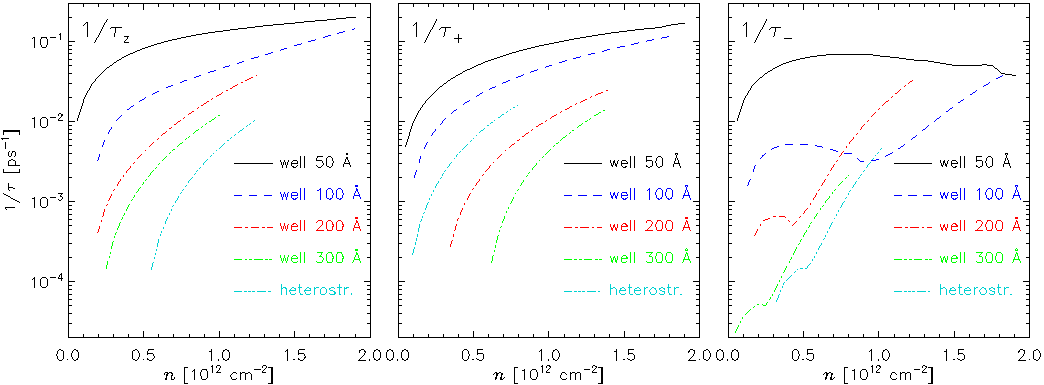
\includegraphics[width=\textwidth]{bigfig}

  \caption{\label{fig:sidewaysF}A big figure that needs to go
   sideways.}
\end{sidewaysfigure}

\section{The End}
\label{sec:end}

Finally, this is the end.  The bibliography starts on
the next page.

%%%%%%%%%%%%%%%%%%%%%%%%%%%%%%%%%%%%%%%%%%%%%%%%%%%%%%%%%%%%%%%%%%

%%% Local Variables: 
%%% TeX-master: "mythesis"
%%% End: 
		% file with Chapter 2 contents
%% This defines the bibliography file (main.bib) and the bibliography style.
%% If you want to create a bibliography file by hand, change the contents of
%% this file to a `thebibliography' environment.  For more information 
%% see section 4.3 of the LaTeX manual.
\begin{doublespace}
\nocite{*}
\bibliography{main}
\bibliographystyle{plain}
\end{doublespace}
		% file with references

%%%%%%%%%%%%%%%%%%%%%%%%%%%%%%%%%%%%%%%%%%%%%%%%%%%%%%%%%%%%%%%%%%%
%%  Appendices

\appendix
\chapter{Objective Symptoms}
% \OnePageChapter	% (use if this chapter/appendix is 1 page long)

Appendices follow the same page-numbering rules as regular chapters. The first
page of a multi-page appendix is not numbered. But the page of a
single-page appendix {\em is} numbered.

\textbf{Are they slow learners} or is it a \emph{REAL} problem?
These are classic findings in the hopelessly computer challenged.

\begin{enumerate}

\item  Can't copy from hard drive to disk.
\item  Can't eject disks.
\item  The word ``disk'' has thousands of meanings to them. None are correct.
\item  Saving a document in any form is a concept totally unexplainable to them.
\item  Desktop covered with Untitled Folders - look again,
		untitled folders are everywhere.
\item  ``Lost'' documents found often in the Apple Menu.
\item  Trash always full. Claim they don't know how to place things in trash.
\item  Mysterious things happen to their documents or computer
	when they are not present.  AKA ``computer victims''.
\item  Highlighting = deleting. Dragging = Oblivion.
\item  Selecting, double-clicking a problem?
		They will always say their mouse is broken.
\item  Their double- click mechanics wants you to send them to a neurologist.
\item  Computer always on due to fear of having to restart it.
\item  Have never read their QuickMail - will say ``I prefer a phone call''.
\item  Have magical beliefs about what computers do.
\item  Describes some flaky way computers could REALLY help them,
		but is not yet available.
\item  Constantly saying they need more ``memory''.
\item  Requests gizmos and gadgets, i.e., ``mouse leash'' or ``disk cozy''.
\item  Avoids eye contact when talking about computers.

\end{enumerate}
			% file with Appendix A contents
\chapter{Ode to Spot}

\noindent\paragraph{(Data, Stardate 1403827)}
Throughout the ages, from Keats to Giorchamo, poets have
composed ``odes'' to individuals who have had a profound effect
upon their lives.  In keeping with that tradition
I have written my next poem \ldots in honor of my cat.
I call it\ldots{}Ode\ldots{}to Spot.
(Shot of Geordi and Worf in audience,
looking mystified at each other.)

\begin{quotation}
\noindent Felus cattus, is your taxonomic nomenclature \\
an endothermic quadruped, carnivorous by nature? \\
Your visual, olfactory, and auditory senses \\
contribute to your hunting skills, and natural defenses. \\
I find myself intrigued by your sub-vocal oscillations, \\
a singular development of cat communications \\
that obviates your basic hedonistic predilection \\
for a rhythmic stroking of your fur to demonstrate affection. \\
A tail is quite essential for your acrobatic talents; \\
you would not be so agile if you lacked its counterbalance. \\
And when not being utilized to aid in locomotion, \\
It often serves to illustrate the state of your emotion.
\end{quotation}


\noindent(Commander Riker begins to applaud, until a
glance from Counselor Troi brings him to a halt.)
Commander Riker, you have anticipated my denouement.
However, the sentiment is appreciated.  I will continue.


\begin{quotation}
\noindent O Spot, the complex levels of behavior you display \\
connote a fairly well-developed cognitive array. \\
And though you are not sentient, Spot, and do not comprehend \\
I nonetheless consider you a true and valued friend.
\end{quotation}
			% file with Appendix B contents

\end{document}
